\graphicspath{{ch5_tist/}{figures/}}
% \graphicspath{{Figures/}}

\chapter{Domain Adaptation for Medical Image Segmentation using Transformation-Invariant Self-Training}
\chaptermark{Domain Adaptation with Transformation-Invariant Self-Training}
\label{chapter:tist}

\sidechaptersummary{Unsupervised Domain Adaptation Method, Transformation Invariant Predictions}

\subsubsection{Synopsis}Models capable of leveraging unlabelled data are crucial in overcoming large distribution gaps between the acquired datasets across different imaging devices and configurations. In this regard, self-training techniques based on pseudo-labeling have been shown to be highly effective for unsupervised domain adaptation. However, the unreliability of pseudo labels can hinder the capability of self-training techniques to induce abstract representation from the unlabeled target dataset, especially in the case of large distribution gaps. 
Since the neural network performance should be invariant to image transformations, we look to this fact to identify uncertain pseudo labels. Indeed, we argue that transformation invariant detections can provide more reasonable approximations of ground truth. Accordingly, we propose an unsupervised domain adaptation strategy termed transformation-invariant self-training (TI-ST) to assess pixel-wise pseudo-labels' reliability and filter out unreliable detections during self-training. We perform comprehensive evaluations for domain adaptation using three different modalities of medical images, two different network architectures, and several alternative state-of-the-art domain adaptation methods. Experimental results confirm the superiority of our proposed method in mitigating the lack of target domain annotation and boosting segmentation performance in the target domain.

\subsubsection{Publication}This chapter is based on a publication\sideauthorcite{ghamsarian2023domain}, and its contents have been modified slightly to be more consistent with the rest of the thesis. In particular, the notation in \Cref{sec:tist_methodology} has been adapted to agree with the rest of the thesis, \Cref{fig:tist_method} has been modified, and \Cref{fig:tist_ablation,fig:ablation_stability} have different colors to those in the published version.

\subsubsection{Author contributions}The work in this chapter was done in collaboration with the University Hospital Bern. The contributing authors were Negin Ghamsarian, Pablo Márquez Neila, Sebastian Wolf, Martin Zinkernagel, Klaus Schoeffmann, and Raphael Sznitman. My contribution consisted of helping with running the experiments and building the figures for the final version of the paper.

\section{Introduction}
\label{sec:full_weakintro}
Semantic segmentation is a fundamental computer vision task with applications in numerous domains such as autonomous driving~\sidecite{cordts2016cityscapes,siam2017deep}, scene understanding~\sidecite{sless2019road}, surveillance~\sidecite{tseng2021person} and medical diagnosis~\sidecite{chen2020deep,hesamian2019deep}. As the advent of deep learning has significantly advanced the state-of-the-art, many new application areas have come to light and continue to do so too. This growth has brought and continues to bring exciting domain-specific datasets for segmentation tasks~\sidecite{islam2020semantic,li2020mas3k,Bodenstedt2018,liu2020fsd,WelinderEtal2010}. 

Today, the process of establishing machine learning-based segmentation models for any new application is relatively well understood and standard. Only once an image dataset is gathered and curated, can machine learning models be trained and validated. In contrast, building appropriate datasets is known to be difficult, time-consuming, and yet paramount. Beyond the fact that collecting images can be tedious, a far more challenging task is producing ground-truth segmentation annotations to subsequently train (semi) supervised machine learning models. This is mainly because producing segmentation annotations often remains a manual task. As reported in~\sidecite{Bearman16}, generating segmentation annotations for a single PASCAL image~\sidecite{pascal-voc-2012} takes over 200 seconds on average. This implies over 250 hours of annotation time for a dataset containing a modest 5'000 images. What often further exacerbates the problem for domain-specific datasets is that only the dataset designer, or a small group of individuals, have enough expertise to produce the annotations (\eg, doctors, experts, etc.), making crowd-sourcing ill-suited. 
%\begin{figure*}[t]
%\centering
%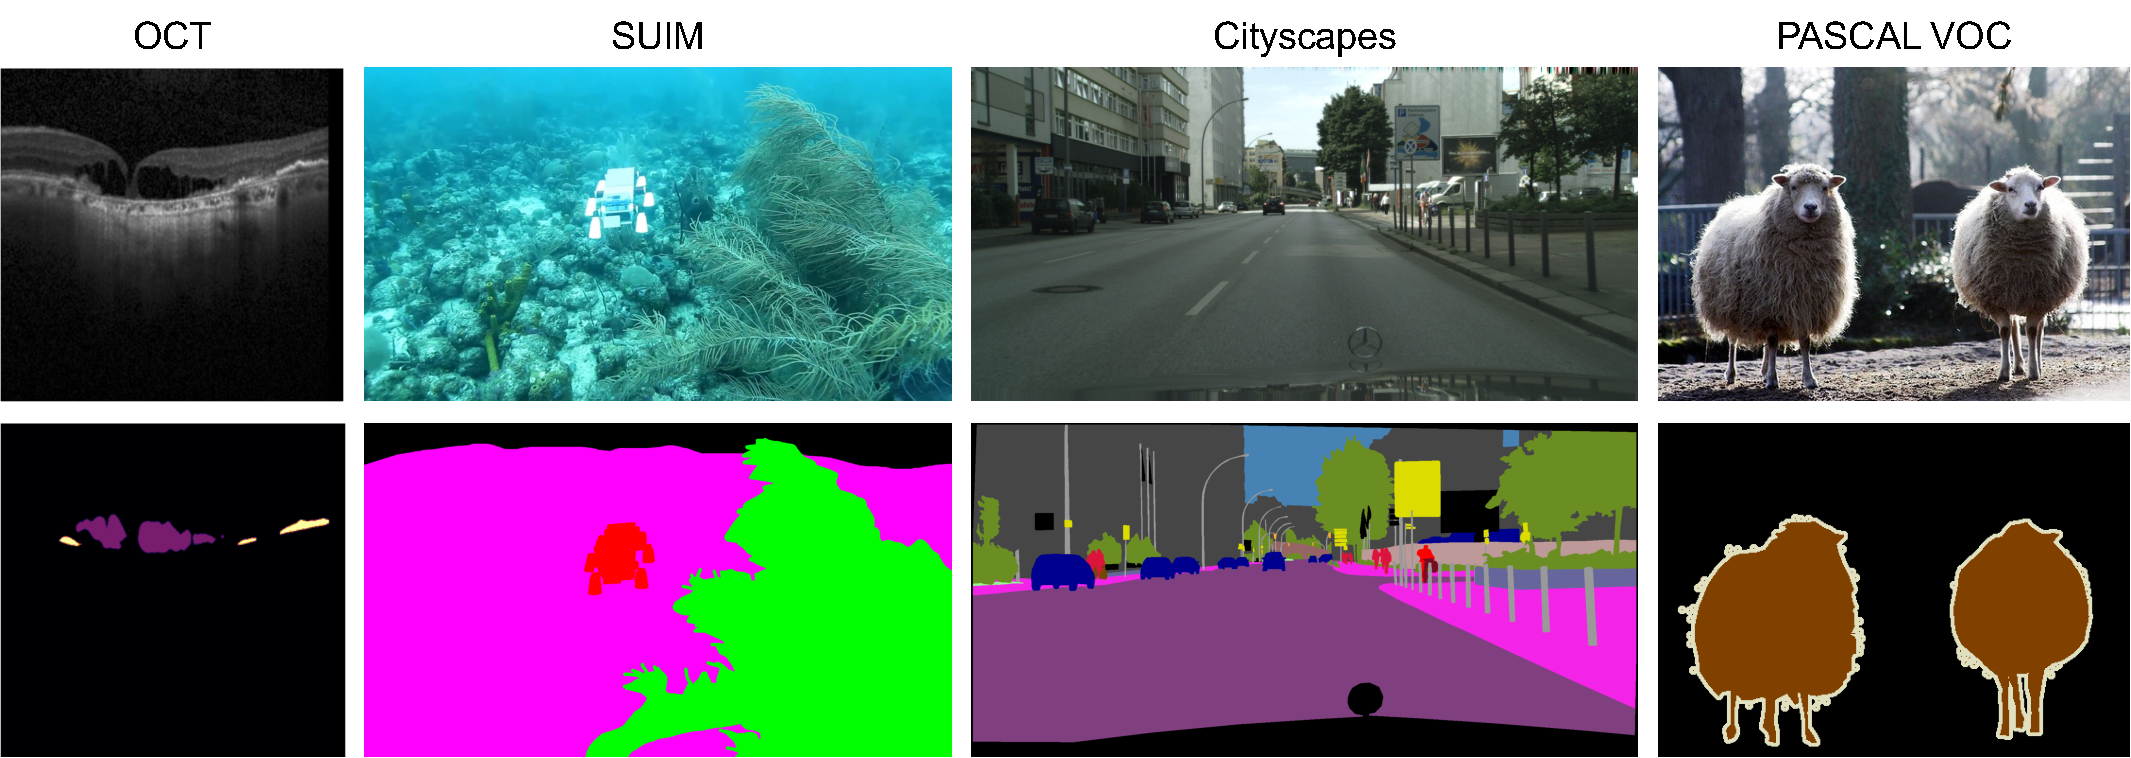
\includegraphics[width=0.99\textwidth]{Figures/datasets.pdf}
%\caption{Illustration of different semantic segmentation applications; OCT: Pathologies of the eye in OCT images, SUIM: Underwater scene segmentation~\sidecite{islam2020semantic}, Cityscape: street level scene segmentation~\sidecite{cordts2016cityscapes}, PASCAL VOC: natural object segmentation.}
%\label{fig:datasets}
%\end{figure*}

\plainwidefig[t]{1}{Figures/datasets.pdf}{Illustration of different semantic segmentation applications; OCT: Pathologies of the eye in OCT images, SUIM: Underwater scene segmentation~\cite{islam2020semantic}, Cityscape: street level scene segmentation~\cite{cordts2016cityscapes}, PASCAL VOC: natural object segmentation.}{fig:fullweak_datasets}

To overcome this challenge, different paradigms have been suggested over the years. Approaches such as Active Learning~\sidecite{Cai21,Casanova2020Reinforced,Konyushkova15} aim to iteratively identify subsets of images to annotate so as to yield highly performing models. Transfer learning has also proved to be an important tool in reducing annotation tasks~\sidecite{Ding2019,heker2020joint,kolesnikov2020big,koleshnikov2021,Liang2020,menegola2017}. For instance, \sidecite{Mensink}~show that training segmentation models from scratch is often inferior to using pre-training models derived from large image classification datasets, even when the target application domain differs from the source domain. Finally, weakly-supervised methods~\sidecite{ahn2018learning,Papandreou15} combine pixel-wise annotations with other weak annotations that are faster to acquire, thereby reducing the annotation burden. In particular, Papandreou~\etal~\sidecite{Papandreou15} showed that combinations of strong and weak annotations (\eg, bounding boxes, keypoints, or image-level tags) delivered competitive results with a reduced annotation effort. In this work, we rely on these observations and focus on the weakly supervised segmentation setting.


In the frame of designing annotation campaigns, weakly-supervised approaches present opportunities for efficiency as well. Instead of completely spending a budget on a few expensive annotations, weakly-supervised methods allow a proportion of the budget to be allocated to inexpensive, or weak, labels. That is, one could spend the entire annotation budget to manually segment available images, but would ultimately lead to relatively few annotations. Conversely, weak annotations such as image-level labels are roughly 100~times cheaper to gather than their segmentation counterparts~\sidecite{Bearman16}. Thus, a greater number of weakly-annotated images could be used to train segmentation models at an equal cost. In fact, under a fixed budget, allocating a proportion of the budget to inexpensive image-level class labels has been shown to yield superior performance compared to entirely allocating a budget to segmentation labels~\sidecite{Bearman16}.

Yet, allocating how an annotation budget should be distributed among strong and weak annotations is challenging, and inappropriate allocations may severely impact the quality of the final segmentation model. For example, spending the entire budget on image-level annotations will clearly hurt the performance of a subsequent segmentation model. Instead, a naive solution would be to segment and classify a fixed proportion of each \sidenote{\eg, 80\% of the budget allocated for segmentation annotations and 20\% for classification.}. Knowing what proportion to use for a given dataset is unclear, however. Beyond this, there is no reason why the same fixed proportion would be appropriate across different datasets or application domains. That is, it would be highly unlikely that the datasets shown in \cref{fig:fullweak_datasets} all require the same proportion of strong and weak annotations to yield optimal segmentation models.

Despite its importance, choosing the best proportion of annotation types remains a largely unexplored research question. Weakly-supervised and transfer-learning methods generally assume that the annotation campaign and the model training are independent and that all annotations are simply available at training time. While active learning methods do alternate between annotation and training, they focus on choosing optimal samples to annotate rather than choosing the right type of annotations. Moreover, most active learning methods ignore constraints imposed by an annotation budget. More notable, however, are the recent works of Mahmood {\it et.~al.}~\sidecite{mahmood2022, mahmood2022optimizing} which aim to determine what weak and strong annotation strategy is necessary to achieve a target performance level. While noteworthy, this objective differs from that here, whereby given a fixed budget, what strategy is best suited for a given new dataset?

To this end, we propose a novel method to find an optimal budget allocation strategy in an online manner\sidedef{online learning}{The data is accessible in a sequential order and is employed to update the model at each step.}. Using a collection of unlabeled images and a maximum budget, our approach selects strong and weak annotations, constrained by a given budget, that maximize the performance of the subsequent trained segmentation model. To do this, our method iteratively alternates between partial budget allocations, label acquisition, and model training. At each step, we use the annotations performed so far to train multiple models to estimate how different proportions of weak and strong annotations affect model performance. A Gaussian Process models these results and maps the number of weak and strong annotations to the expected model improvement. Computing the Pareto optima between expected improvement and costs, we choose a new sub-budget installment and its associated allocation so to yield the maximum expected improvement. We show in our experiments that our approach is beneficial for a broad range of datasets, and illustrate that our dynamic strategy allows for high performances, close to optimal fixed strategies that cannot be determined beforehand.

\section{Methodology}
\label{sec:tist_methodology}

Consider a labeled source dataset, $\mathcal{S}$, with training images $\mathcal{X_S}$ and corresponding segmentation labels $\mathcal{Y_S}$, while we denote a target dataset $\mathcal{T}$, containing only target images $\mathcal{X_T}$. We aim to train a network using $\mathcal{X_S}$, $\mathcal{Y_S}$, and $\mathcal{X_T}$ for semantic segmentation in the target dataset. 


We propose to train the model using a self-supervised approach on the images $\mathcal{X_T}$ by assigning pseudo labels during training. Typical pseudo labels are computed from independent predictions of unlabeled images. Instead, our proposed framework adopts a self-assessment strategy to determine the reliability of predictions in an unsupervised fashion. Specifically, we propose to target highly-reliable predictions generated by a network aiming for transformation-invariant confidence. Compared to self-ensembling strategies that penalize the distant predictions corresponding to the transformed versions of identical inputs, our goal is to filter out transformation-variant predictions. Indeed, our method reinforces the ensemble of high-confidence predictions from two versions of the same target sample. Our proposed TI-ST framework simultaneously trains on the source and target domains, so as to progressively bridge the intra-domain distribution gap. \cref{fig:BD} depicts our TI-ST framework, which we detail in the following sections. 

%\begin{figure}[t]
%\centering
%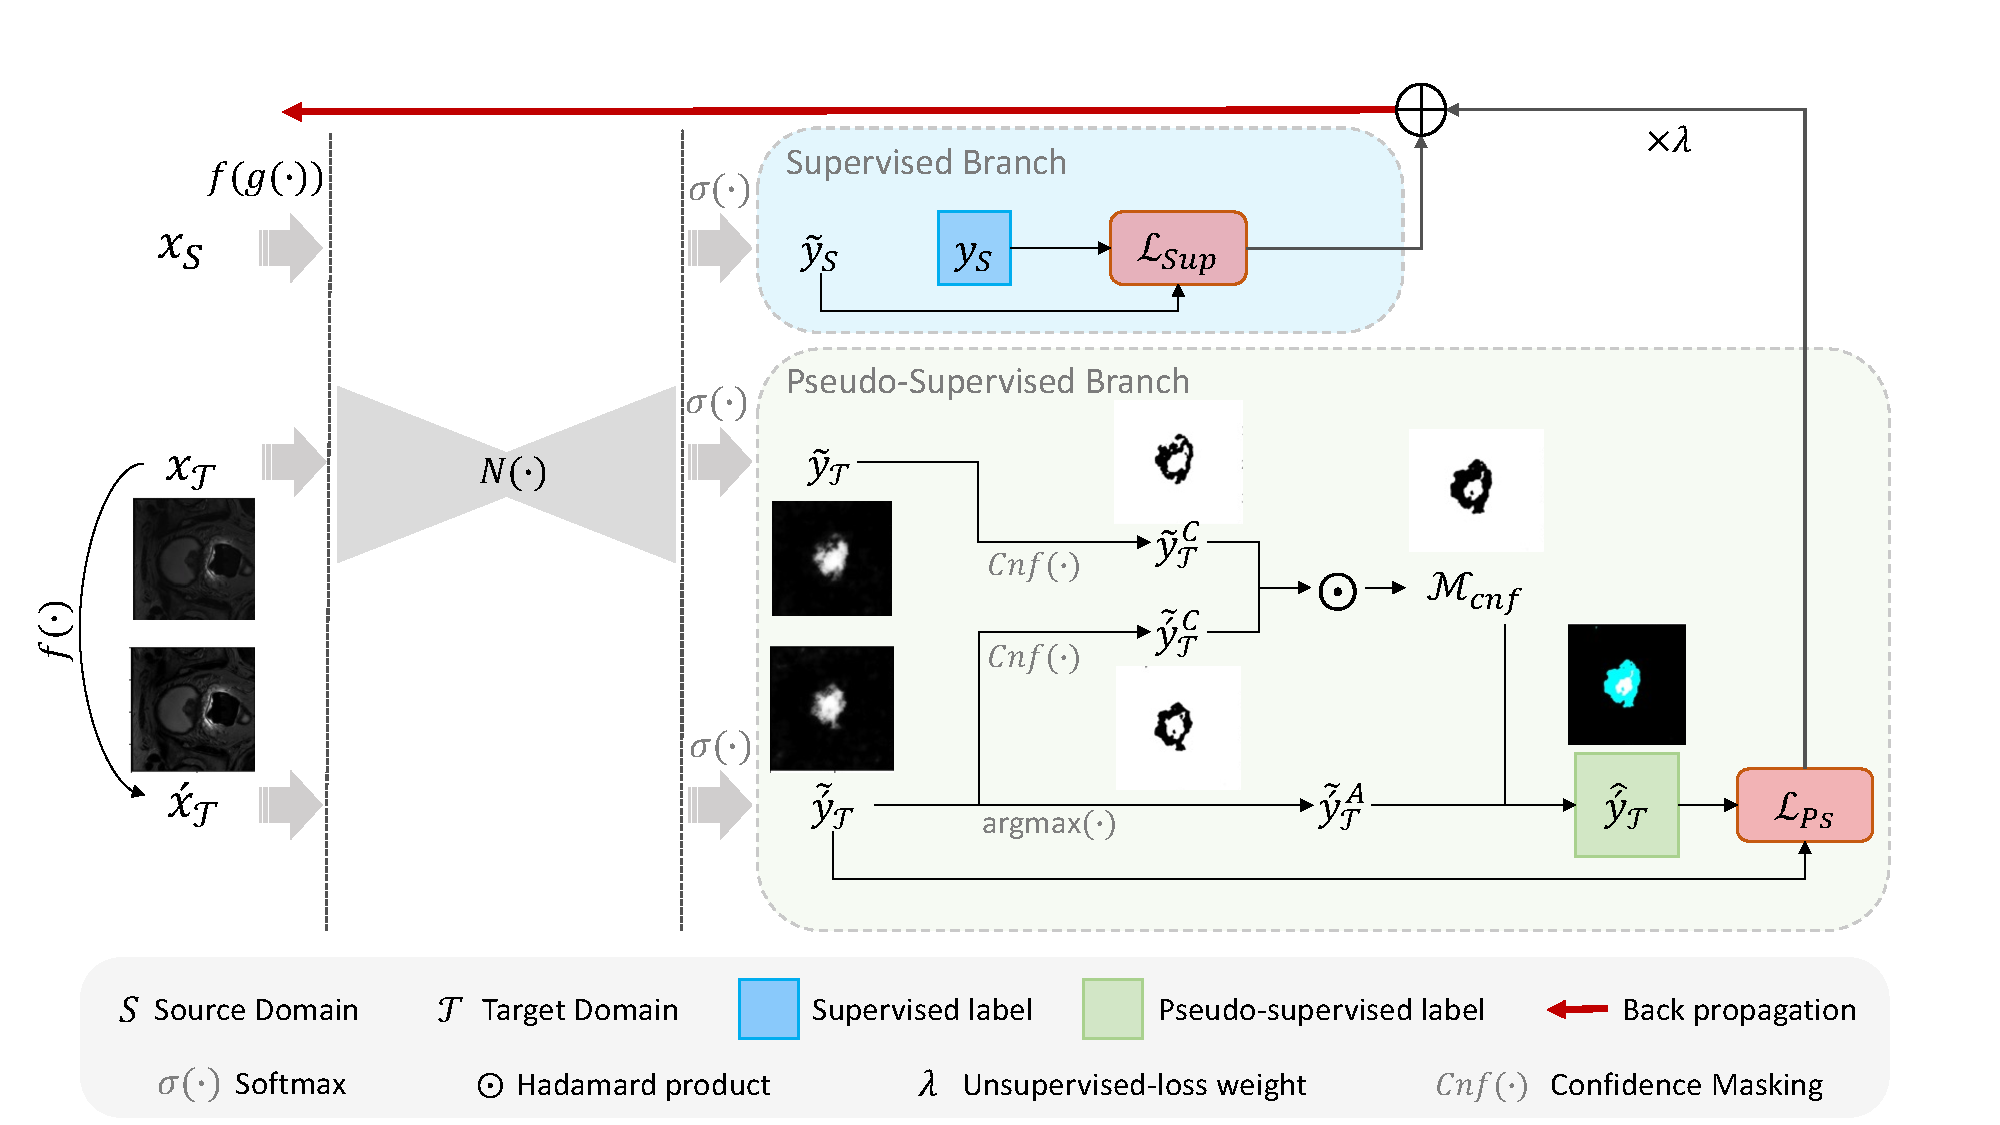
\includegraphics[width=\textwidth]{figures/BD8.pdf}
%\caption{Proposed unsupervised domain adaptation framework based on transformation-invariant self-training (TI-ST). Ignored pseudo-labels during unsupervised loss computation are shown in turquoise.
%}
%\label{fig:BD}
%\end{figure}

\plainwidefig{1}{figures/BD8.pdf}{Proposed unsupervised domain adaptation framework based on transformation-invariant self-training (TI-ST). Ignored pseudo-labels during unsupervised loss computation are shown in turquoise.}{fig:BD}

\subsection{Model} At training time, images from the source dataset are augmented using spatial $g(\cdot)$ and non-spatial $f(\cdot)$ transformations and passed through a segmentation network, $N(\cdot)$, by which the network is trained using a standard supervision loss. At the same time, images from the target dataset are also passed to the network. Specifically, we feed two versions of each target image to the network: (1) the original target image $x_\mathcal{T}$, and (2) its non-spatially transformed version, $\Acute{x_\mathcal{T}} = f(x_\mathcal{T})$. 
% \RS{There is no other mention of $f$ throughout the method. We should probably give some information as to what we use, and why.} 
Once fed through the network, the corresponding predictions can be defined as $\tilde{y_{\mathcal{T}}} = \sigma(N(x_{\mathcal{T}}))$ and $\tilde{\acute{y_{\mathcal{T}}}} = \sigma(N(\Acute{x_{\mathcal{T}}}))$, where $\sigma(\cdot)$ is the Softmax operation. We then define a confidence-mask ensemble as
\begin{equation}
\mathcal{M}_{cnf} = 
Cnf(\tilde{{y_{\mathcal{T}}}})
\odot
Cnf(\tilde{\Acute{y_{\mathcal{T}}}}),
\label{eq: ensemble of confidence}
\end{equation}
\noindent
where $\odot$ refers to Hadamard product used for element-wise multiplication, and $Cnf$ is the high confidence masking function,
\iffalse
\begin{equation}
    \mathcal{M}_{cnf}(\tilde{\acute{y_T}}, \Acute{\tilde{y_T}}) = h(\tilde{\acute{y_T}})\odot h(\Acute{\tilde{y_T}})
    \label{eq: confidence mask}
\end{equation}
\fi
\begin{equation}
    Cnf_{\textsub{$\in (W\times H$)}}(y) =
    \begin{cases}
    0, & \text{if    } \maxH_{\textsub{C}}(y) > \uptau\\
    1, & \text{else.  }
    \end{cases}
    \label{eq: filtering}
\end{equation}
\noindent
where $\uptau \in (0.5,1) $ is the confidence threshold, and $H$, $W$, and $C$ are the height, width, and number of classes in the output, respectively. Specifically, $\mathcal{M}_{cnf}$ encodes regions of confident predictions that are invariant to transformations.
We can then compute the pseudo-ground-truth mask for each input from the target dataset as
\begin{equation}
\hat{\Acute{y_{\mathcal{T}}}} = 
\begin{cases}
\argmaxH_{\textsub{C}} (\tilde{\Acute{y_{\mathcal{T}}}}), & \text{if  } \:\mathcal{M}_{cnf} = 1\\
\text{ignore}, & \text{else.  }
\end{cases}
\end{equation}
\noindent

\subsection{Training}
To train our model, we simultaneously consider both the source and target samples by minimizing the following loss,
\begin{equation}
    \mathcal{L}_{overall} = \mathcal{L}_{Sup}( \tilde{y_\mathcal{S}}, y_\mathcal{S}) + \lambda \Big(\mathcal{L}_{Ps}(\mu (\tilde{\Acute{y_{\mathcal{T}}}}), \hat{\Acute{y_{\mathcal{T}}}})\Big) ,
    \label{eq: loss}
\end{equation}
\noindent
where $\mathcal{L}_{Sup}$ and $\mathcal{L}_{Ps}$ indicate the supervised and pseudo-supervised loss functions used, respectively. We set $\lambda$ as a time-dependent weighing function that gradually increases the share of pseudo-supervised loss. Intuitively, our pseudo-supervised loss enforces predictions on transformation-invariant highly-confident regions for unlabeled images. 

\subsubsection{Discussion} 
The quantity and distribution of supervised data are determining factors in neural networks' performance. With highly distributed large-scale supervisory data, neural networks converge to an optimal state efficiently. However, when only limited supervisory data, with heterogeneous distribution from the inference dataset, using more sophisticated methods to leverage a priori knowledge is essential. Our proposed use of invariance of network predictions with respect to data augmentation is a strong form of knowledge that can be learned through dataset-dependent augmentations. The trained network is then expected to provide consistent predictions under diverse transformations. Hence, the transformation variance of the network predictions can indicate the network's prediction doubt and low confidence correspondingly. We take advantage of this characteristic to assess the reliability of predictions and filter out unreliable pseudo-labels.\jgt{Check all this paragraph}

\section{Experimental setup}
\label{sec:tist_experimental_settings}

\subsection{Datasets}
We validate our approach on three cross-device/site datasets for three different modalities: 

\begin{itemize}
    \item \textbf{Cataract:} instrument segmentation in cataract surgery videos. We set the ``Cat101''~\sidecite{cat101} as the source dataset and the ``CaDIS'' as the target domain dataset~\sidecite{CaDIS}. 
    \item \textbf{OCT:} IRF Fluid segmentation in retinal OCTs~\sidecite{retouch}. We use the high-quality ``Spectralis'' dataset as the source and the lower-quality ``Topcon'' dataset as the target domain.
    \item \textbf{MRI:} multi-site prostate segmentation~\sidecite{liu2020ms}. We sample volumes from ``BMC'' and ``BIDMC'' as the source and target domain, respectively\sidenote{``BIDMC'' imposes a more challenging scenario than ``BMC'' due to the low contrast of the images.}.
\end{itemize} 

We follow a four-fold validation strategy for all three cases and report the average results over all folds. The average number of labeled training images (from the source domain), unlabeled training images (from the target domain), and test images per fold are equal to ($207, 3'189,58$) for Cataract, ($391,569,115$) for OCT, and ($273,195,65$) for MRI dataset.

\subsection{Baseline methods}
We compare the performance of our proposed transformation-invariant self-training (SI-ST) method against seven state-of-the-art alternative methods that represent different domain adaptation methods and paradigms: $\Uppi$ models~\sidecite{TESSL}, temporal ensembling~\sidecite{TESSL}, mean teacher~\sidecite{UDAMIS}, cross pseudo supervision (CSP)~\sidecite{CPS}, reciprocal learning (RL)~\sidecite{Reciprocal} and self-training (ST)~\sidecite{st++}.

\subsection{Networks and training settings}
We evaluate our TI-ST framework using two different architectures:  (1) DeepLabV3+~\sidecite{DeepLabV3} with ResNet50 backbone~\sidecite{ResNet} and (2) scSE~\sidecite{SCSE} with VGG16 backbone. Both backbones are initialized with the ImageNet~\sidecite{deng2009imagenet} pre-trained parameters. We use a batch size of four for the Cataract and MRI datasets and a batch size of two for the OCT dataset. For all training strategies, we set the number of epochs to 100. The initial learning rate is set to 0.001 and decayed by a factor of $0.8$ every two epochs. The input size of the networks is $512\times 512$ for cataract and OCT and $384\times 384$ for the MRI dataset. 
As spatial transformations $g(\cdot)$, we apply cropping and random rotation (up to 30 degrees). 

The non-spatial transformations, $f(\cdot)$, include color jittering (brightness = 0.7, contrast = 0.7, saturation = 0.7), Gaussian blurring, and random sharpening. The confidence threshold $\uptau$ for the self-training framework and the proposed TI-ST framework is set to $0.85$ except in the ablation studies\sidenote{See \Cref{sec:experimental_results_tist}}. In Eq.~\eqref{eq: loss}, the weighting function $\lambda$ ramps up from the first epoch along a Gaussian curve equal to $\exp[-5(1-\text{current-epoch}/{\text{total-epochs}})]$. The unsupervised loss is set to the \autoindex{cross-entropy loss}, and the supervised loss is set to the \textit{cross entropy log dice} loss, which is a weighted sum of cross-entropy and the logarithm of soft dice coefficient. For the TI-ST framework, we only use non-spatial transformations for the self-training branch for simplicity.


\section{Results}
\label{sec:experimental_results_tist}

\begin{table}[t]
\centering

% @{}lccccccc@{}
%\begin{tabular}{lm{1.3cm}m{1.3cm}m{1.3cm}m{1.3cm}m{1.3cm}m{1.3cm}m{1.3cm}}
\begin{tabular}{lm{1.3cm}*{7}{>{\centering\arraybackslash}m{1.3cm}}}
\toprule
Modality & \multicolumn{2}{c}{\footnotesize{Cataract Surgery}} & \multicolumn{2}{c}{\footnotesize{OCT}} & \multicolumn{2}{c}{\footnotesize{MRI}} & \multicolumn{1}{l}{\multirow{2}{*}{\footnotesize{Avg. Rel.}}} \\ \cmidrule(lr){2-3}\cmidrule(lr){4-5}\cmidrule(lr){6-7}
Network & \footnotesize{DLV3+} & \footnotesize{scSENet} & \footnotesize{DLV3+} & \footnotesize{scSENet} & \footnotesize{DLV3+} & \footnotesize{scSENet} &   \\ \midrule
Supervised & 15.42 & 37.67 & 22.87 & 24.08 & 52.39 & 65.93 & N/A \\
$\Uppi$ Model~\cite{TESSL} & 27.55 & 35.56 & 1.12 & 0.00 & 10.00 & 6.87 & -22.88 \\
TE~\cite{TESSL} & 33.10 & 42.32 & 42.13 & 39.86 & 63.41 & 67.25 & 11.62 \\
Mean Teacher~\cite{UDAMIS} & 11.06 & 39.54 & 19.11 & 4.70 & 64.82 & 66.87 & -2.04 \\
RL~\cite{Reciprocal} & 34.40 & 45.13 & 48.73 & 47.70 & 60.79 & 70.20 & 14.77 \\
CPS~\cite{CPS} & 36.24 & 39.40 & 47.31 & 14.71 & 76.00 & 68.80 & 10.68 \\
ST~\cite{st++} & 34.34 & 41.10 & 36.84 & 33.01 & 68.63 & 71.97 & 11.26 \\\midrule
% ST++~\cite{st++} &  &  &  &  &  &  &  \\
{\bf TI-ST} & 37.69 & 45.31 & 50.93 & 40.87 & 66.56 & 74.07 & 16.18 \\ 
& \textcolor{gray}{\scriptsize{(+22.27)}} & \textcolor{gray}{\scriptsize{(+7.46)}} & \textcolor{gray}{\scriptsize{(+28.06)}} & \textcolor{gray}{\scriptsize{(+16.79)}} & \textcolor{gray}{\scriptsize{(+14.17)}} & \textcolor{gray}{\scriptsize{(+8.14)}}\\
\bottomrule
\end{tabular}
\sidecaption{Quantitative comparisons in Dice score (\%) among the proposed (TI-ST) and alternative methods for DeepLabV3+~\cite{DeepLabV3} (DLV3+) and scSENet~\cite{SCSE} and the three datasets. Relative Dice computed over the Supervised baseline. \label{tab:quantitative}}


\end{table}


\cref{tab:quantitative} lists the performance of our transformation-invariant self-training (TI-ST) approach with alternative methods across the three tasks and using two network architectures. According to the quantitative results, TI-ST, RL, ST, and CPS are the best-performing methods. Nevertheless, our proposed TI-ST achieves the highest average relative improvement in dice score compared to naive supervised learning ($16.18\%$ average improvement). Considering our main competitor (RL), we note that our proposed TI-ST method is a one-stage framework using one network. In contrast, RL is a two-stage framework (requiring a pre-training stage) and uses a teacher-student network. Hence, TI-ST is also more efficient than RL in terms of time and computation.  Furthermore, the proposed strategy demonstrates the most consistent results when evaluated on different tasks, regardless of the utilized neural network architecture. 

\textfig{1}{figures/ablationf.pdf}{Ablation studies on the pseudo-labeling threshold and size of the labeled dataset.}{fig:ablation}

\cref{fig:ablation}-(a-b) demonstrates the effect of the pseudo-labeling threshold on TI-ST performance compared with regular ST. We observe that filtering out unreliable pseudo-labels based on transformation variance can remarkably boost pseudo-supervision performance regardless of the threshold. \cref{fig:ablation}-(c) compares the performance of the supervised baseline, ST, and TI-ST with respect to the number of source-domain labeled training images. While ST performance converges when the number of labeled images increases, our TI-ST pushes decision boundaries toward the target domain dataset by avoiding training with transformation variant pseudo-labels. We validate the stability of TI-ST vs. ST  with different labeling thresholds (0.80 and 0.85) over four training folds in \cref{fig:ablation_stability}, where TI-ST achieves a higher average improvement relative to supervised learning for different tasks and network architectures. This analysis also shows that the performance of ST is sensitive to the pseudo-labeling threshold and generally degrades by reducing the threshold due to resulting in wrong pseudo labels. However, TI-ST can effectively ignore false predictions in lower thresholds and take advantage of a higher amount of correct pseudo labels. This superior performance is depicted qualitatively in \cref{fig:qualitative}.

%\begin{figure}[b]
%\centering
%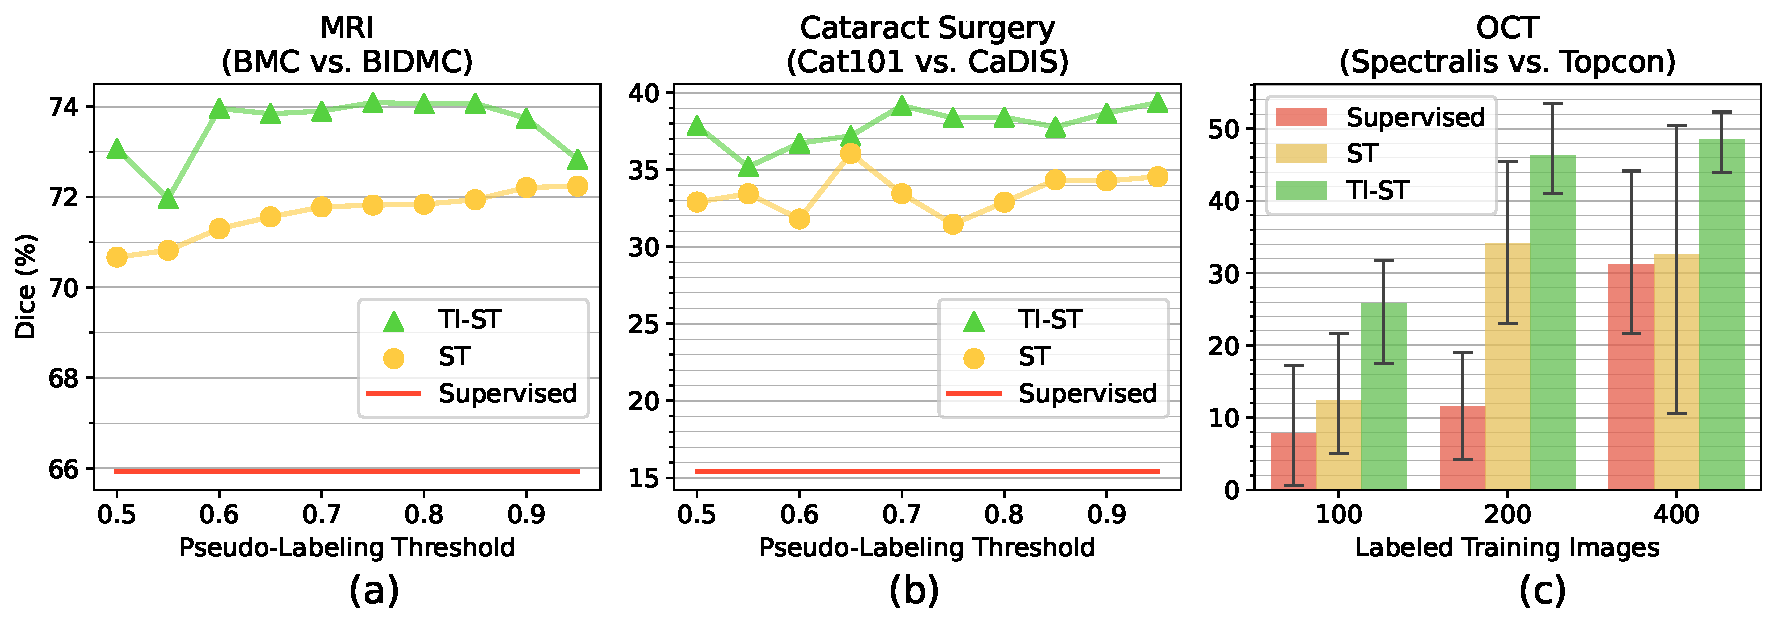
\includegraphics[width=1\textwidth]{figures/ablationf.pdf}
%\sidecaption{Ablation studies on the pseudo-labeling threshold and size of the labeled dataset. 
%}
%\label{fig:ablation}
%\end{figure}




%\begin{figure}[t]
%\centering
%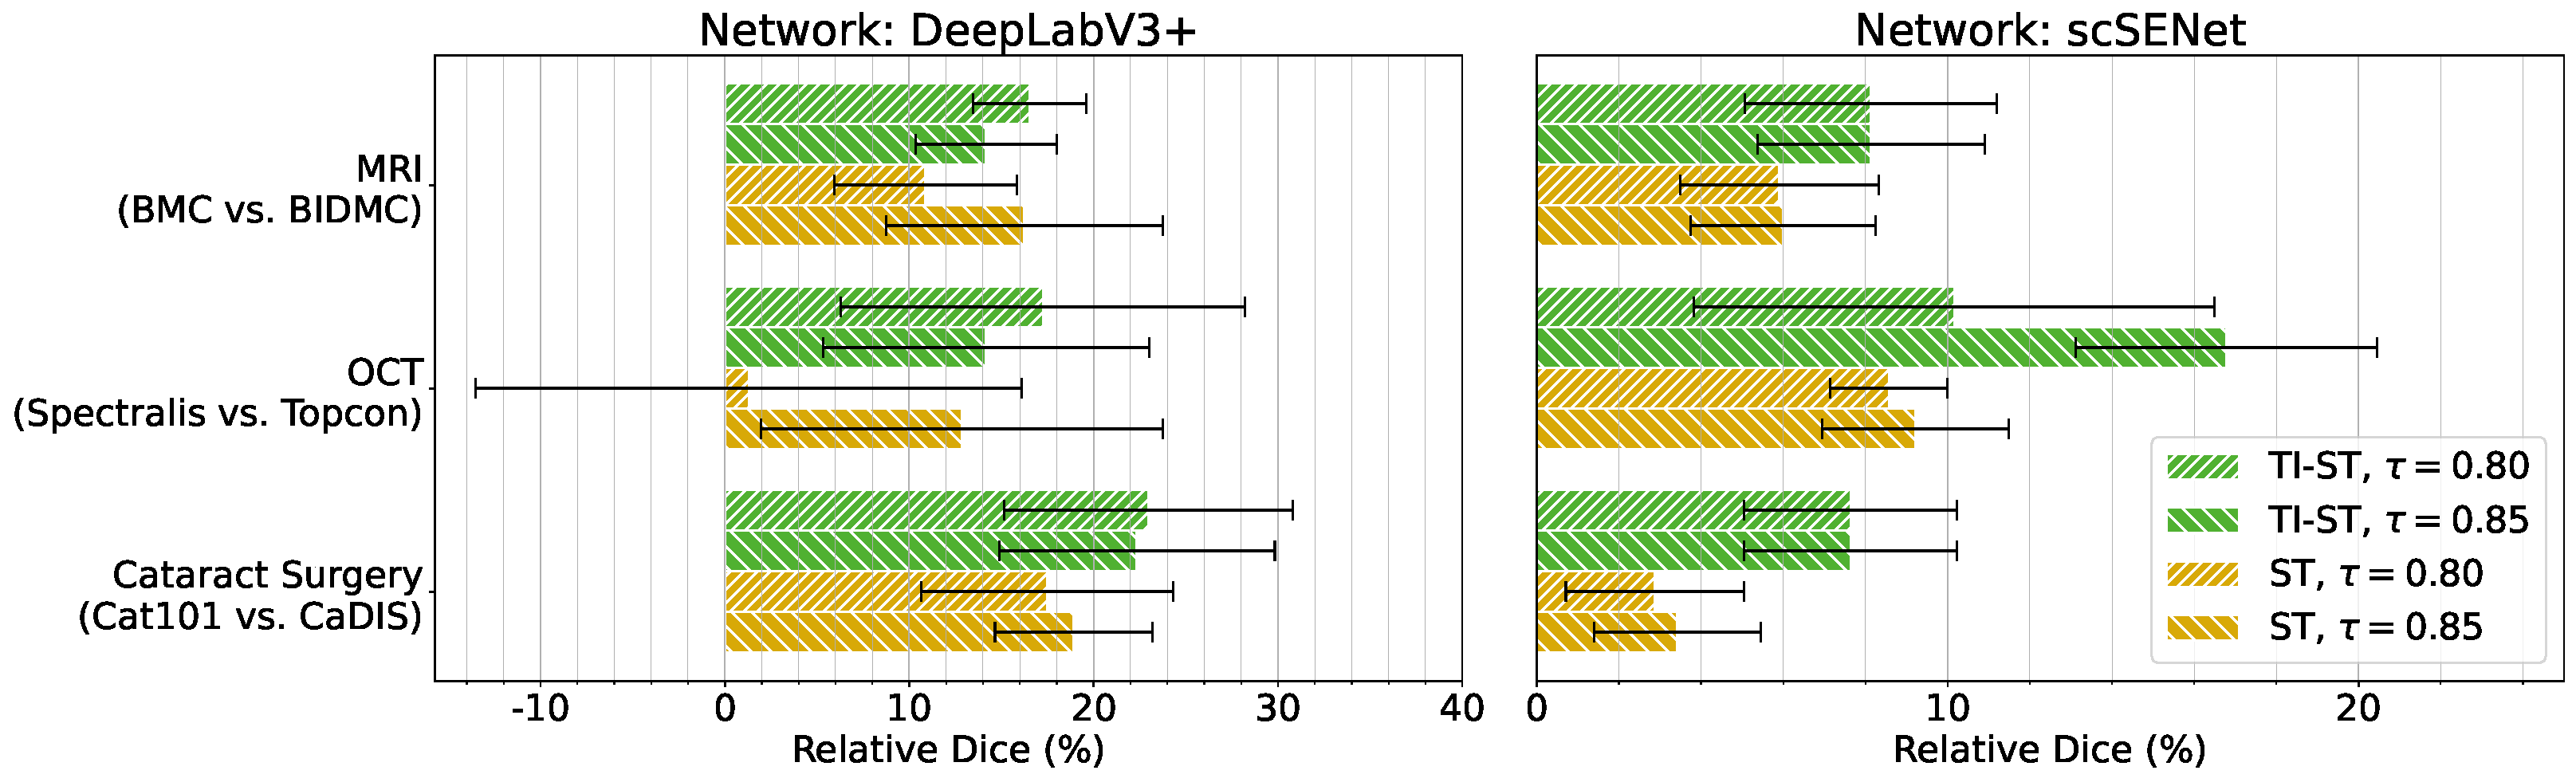
\includegraphics[width=1\textwidth]{figures/ablation_stability10.pdf}
%\caption{Ablation study on the performance stability of TI-ST vs. ST across the different experimental segmentation tasks.
%}
%\label{fig:ablation_stability}
%\end{figure}

\textfig{1}{figures/ablation_stability10.pdf}{Ablation study on the performance stability of TI-ST vs. ST across the different experimental segmentation tasks.}{fig:ablation_stability}

%\begin{figure}[t]
%\centering
%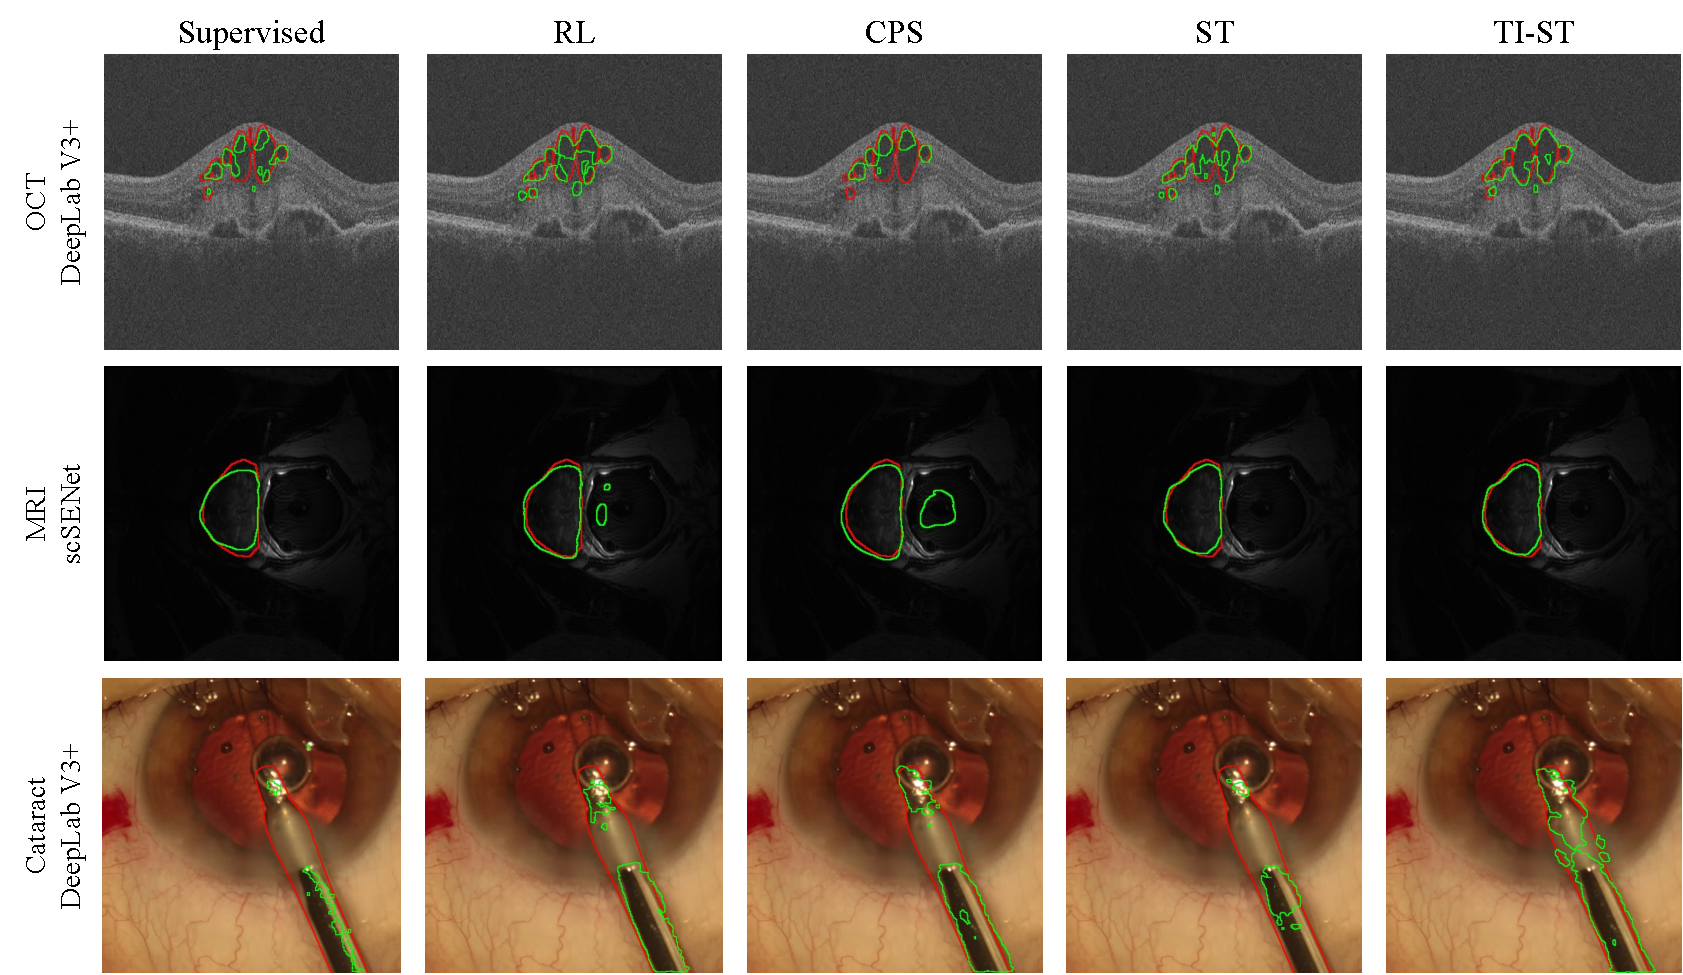
\includegraphics[width=.9\textwidth]{figures/qualitative.pdf}
%\caption{Qualitative comparisons between the performance of TI-ST and four existing methods.
%}
%\label{fig:qualitative}
%\end{figure}
\widefig{1}{figures/qualitative.pdf}{Qualitative comparisons between the performance of TI-ST and four existing methods.}{fig:qualitative}
\section{Conclusion}
\label{sec:tist_conclusion}

We proposed a novel self-training framework with a self-assessment strategy for pseudo-label reliability, namely ``Transformation-Invariant Self-Training'' (TI-ST). This method uses transformation-invariant highly-confident predictions in the target dataset by considering an ensemble of high-confidence predictions from transformed versions of identical inputs. We experimentally show the effectiveness of our approach against numerous existing methods across three different source-to-target segmentation tasks, and when using different model architectures. Beyond this, we show that our approach is resilient to changes in the methods hyperparameter, making it well-suited for different applications. 